\documentclass[12pt]{article}
\usepackage[utf8]{inputenc}
\usepackage[paperwidth=8.5in, paperheight=25in, margin=1.5in]{geometry}

\usepackage{graphicx}
\usepackage{amsmath}
\usepackage{siunitx}
\numberwithin{equation}{section}
\usepackage{float}
\usepackage{subcaption}
\pagenumbering{gobble} % removes page number from TOC and pages

\usepackage{xcolor}
\definecolor{xlinkcolor}{cmyk}{1,1,0,0}
\usepackage[colorlinks,allcolors=xlinkcolor]{hyperref}
\usepackage[titles]{tocloft} % remove dots in TOC
\renewcommand{\cftdot}{}
\setcounter{tocdepth}{2}

\title{Econometrics}
\author{Andrew Lu}
\date{Mr. Lizardo, Fall 2020}

\begin{document}

    \maketitle
    \label{sec:top}
    \tableofcontents

\section{Introduction to Statistics}

\subsection{Variance}
\begin{align}
    \sigma^2=\frac{\sum\limits_{i=1}^{N}{(x_1-\mu)^2}}{N} \\
    s^2=\frac{\sum\limits_{i=1}^{n}{(x_1-\Bar{x})^2}}{n-1}
\end{align}
where $\sigma^2=$ population variance and $s^2=$ sample variance. The denominator is $n-1$ for sample variance calculations because of degrees of freedom.

\subsection{Standard Deviation}
\begin{align}
    \sigma=\sqrt{\frac{\sum\limits_{i=1}^{N}{(x_1-\mu)^2}}{N}} \\
    s=\sqrt{\frac{\sum\limits_{i=1}^{n}{(x_1-\Bar{x})^2}}{n-1}}
\end{align}

\subsection{Data Distribution}
\subsubsection{Histograms}
\begin{figure}[!ht]
    \centering
    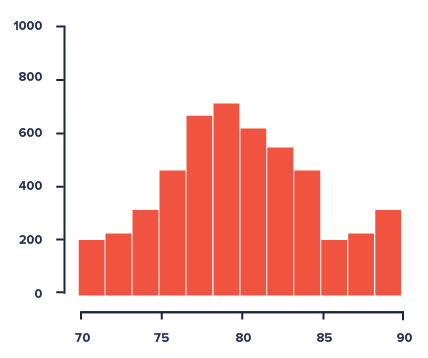
\includegraphics[width=0.6\linewidth]{figures/histogram.png}
\end{figure}
\subsubsection{Box Plots}
\subsubsection{SOCS}
\begin{enumerate}
    \item Symmetry: positive/right skew, negative/left skew, or normal curve
    \item Outliers: skew the distribution in its direction
    \item Center: mean = balancing point, median = data split in half
    \item Spread: outliers affect spread by impacting skew
\end{enumerate}
\begin{figure}[!ht]
    \centering
    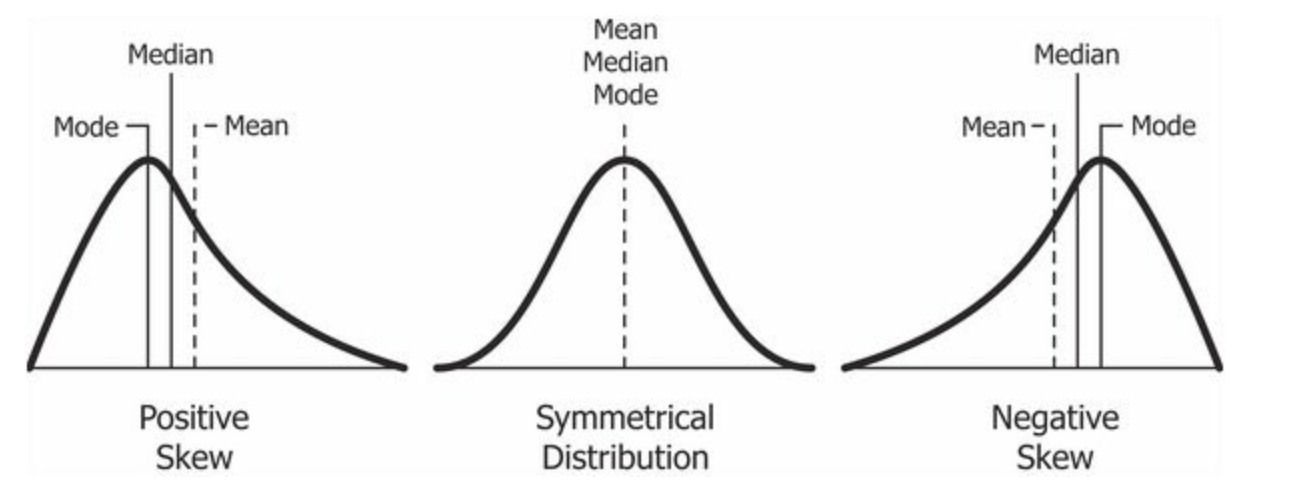
\includegraphics[width=0.9\linewidth]{figures/skew.png}
\end{figure}

\noindent \begin{flushright} \hyperref[sec:top]{back to top} \end{flushright}
\end{document}
